%Note that since this uses BiBTex formatting, if you are using TeXworks to compile this, you need to run (pdflatex-->bibtex-->pdflatex-->pdflatex)

\documentclass[12pt]{article}

\usepackage{amsmath}    % need for subequations
\usepackage{graphicx}   % need for figures
\usepackage{verbatim}   % useful for program listings
\usepackage{color}      % use if color is used in text
\usepackage{subfigure}  % use for side-by-side figures
\usepackage{hyperref}   % use for hypertext links, including those to ext documents and URLs
\usepackage[margin=0.6in]{geometry}
\usepackage{draftmode}		% Draft mode edit;	Remember to remove the linenumbers command

% don't need the following. simply use defaults
\setlength{\baselineskip}{16.0pt}    % 16 pt usual spacing between lines

\setlength{\parskip}{3pt plus 2pt}
\setlength{\parindent}{20pt}
\setlength{\oddsidemargin}{0.5cm}
\setlength{\evensidemargin}{0.5cm}
\setlength{\marginparsep}{0.75cm}
\setlength{\marginparwidth}{2.5cm}
\setlength{\marginparpush}{1.0cm}
\setlength{\textwidth}{150mm}

\begin{comment}
\pagestyle{empty} % use if page numbers not wanted
\end{comment}

% above is the preamble
\linenumbers		% Comment out if not in draftmode
\begin{document}
\begin{center}
{\large \textbf{Standalone ATLAS Analysis Project}} \\
Sam Meehan \footnote{The author can be contacted at \href{mailto:meehan@uchicago.edu}{\textit{meehan@uchicago.edu}} } \\
The University of Chicago \\
High Energy Physics \\


\end{center}

\section{Introduction}
Presently, the LHC is delivering luminosity to ATLAS at a rate of approximately $35 \times 10^{32} \mathrm{cm}^{-2}\mathrm{s}^{-1}$ \footnote{This is as of 19 December 2011 with current running conditions found at \href{http://op-webtools.web.cern.ch/op-webtools/vistar/vistars.php?usr=LHC1}{\textit{http://op-webtools.web.cern.ch/op-webtools/vistar/vistars.php?usr=LHC1}} }.  This luminosity translates into $10^{6}$ collisions per second (That's a lot of collisions).  However, most of these collisions will not be interesting, the definition of which is left up to you.  So it is the job of physicists to develop clever ways to sort through these events and determine interesting signatures that can distinguish the haystack from the needle, unless of course you are looking at the ``haystack", in which case you have a different set of challenges.  \\
\\


However, because of the scale of the ATLAS experiment, the computing infrastructure can take a considerable amount of work to understand and is in such a constant state of flux, that it can be more of a hinderance when working on something like a BA thesis or a summer project.  However, thanks to the work of a lot of smart people, there are analysis tools that can be used to approximate (and they do a pretty good job), the physics that goes on at the LHC using ATLAS.  And the great thing is, these tools can be used on your personal laptop, so you can do LHC physics \textit{anywhere}!!!  This project will introduce you to those tools, help you set them up on your computer \footnote{If you are a student of UC HEP, then work on the local machine \textit{mjolx2}.  This has been configured with proper setups for some of the tools such as Root, python, and the compilers you will need in this project.} \footnote{WARNING: If during this tutorial, you attempt to copy directly from the PDF document, be sure to proofread the code before using it.  Sometimes there are difficulties with reading text from a pdf.}.

\section{Your Project}
%THIS IS JUST AN EXAMPLE AND CAN BE CHANGED TO SUIT THE ROLE OF THE UNDERGRADUATE, BUT THE IDEA WOULD BE TO ONLY HAVE TO CHANGE THIS SECTION AND THE REST OF THE DOCUMENT CAN STAY THE SAME

Within ATLAS, heavy particles, like W and Z bosons, are created in numerous different physics processes including ($q\bar{q}\rightarrow H \rightarrow ZZ^{*}$) and $q\bar{q}\rightarrow Zq\bar{q}$.  But what comes into the ATLAS detector is the decay products of these W and Z bosons.  These decay products can be leptons or partons and we can use the measurements we make of the kinematics of these decay products to reconstruct the W and Z bosons.  Much work has been done to understand the kinematics of leptonically decaying W and Z bosons ~\cite{Wboson_1} ~\cite{Zboson_1} ~\cite{WZboson} ~\cite{WZboson_2}, but those that decay hadronically are more difficult to understand.  This is because the quarks coming from $Z\rightarrow q\bar{q}$ do not interact with the detector in the same way.  In fact they cannot even stay as single quarks because of something called \textit{confinement} ~\cite{confinement}.  Instead, the quarks to \textit{hadronize} and produce a shower of particles that enter into the ATLAS detector calorimeters.  These showers of particles are what we measure and are called \textit{jets} ~\cite{jet_0} ~\cite{jet_1} ~\cite{jet_2} ~\cite{jet_3} ~\cite{jet_4} ~\cite{jet_5}.  In contrast to reconstructing a leptonic decay from clean, well measured electrons or muons, reconstructing a hadronic decay from jets is a much messier business.  For this reason, we are interested in investigating techniques that can be used to extract the most information we can from a jet.  This is a field of study that is called \textit{jet substructure} ~\cite{jetss_1} ~\cite{jetss_2} ~\cite{jetss_3} ~\cite{jetss_4}.  To start with, once you have set up the analysis tools described in the following sections, try to do the following to start your analysis:
\begin{itemize}
  \item You've got a bunch of leptons (electrons and muons) in your ntuple (you'll know what this is later), do all of them fall within the ATLAS detector ~\cite{detector} (think polar angle)?  Do they all have enough energy to be detected?  Put some cuts on kinematic variables to select ``good" leptons.
  \item The ``signal" Monte Carlo that you are working with has the processes $Z\rightarrow \ell \ell$.  By selecting only events with two ``good" leptons, can you reconstruct the invariant mass of the dilepton system and see the leptonically decaying Z boson peak? 
  \item The ``signal" Monte Carlo that you are working with also has the processes $Z\rightarrow qq$.  By selecting only events with two ``good" jets, can you reconstruct their invariant mass and see the hadronically decaying Z boson? 
  \item Which one of these two resonant peaks would be easy to distinguish from a background?  Why? (NOTE: the answer is the leptonically decaying Z peak.  If you don't see this, then ask.)
 \item With MadGraph, produce a large set (1 million) Z+jets events to simulate your background and a large set of ZZ/WZ events where the decay is semileptonic, meaning that the Z decays to $\ell^{+} \ell^{-}$ pair and the other boson decays to a pair of jets.  Analyze both samples in the same way, only selecting events where a good dilepton pair has a mass close to that of the Z boson ($91 \ GeV$) and on the same set of axes, overlay the invariant mass plot of the two highest $p_{T}$ jets, be sure to scale each sample to the corresponding process cross section and luminosity.  If you had data collected from ATLAS, would it be easy to distinguish an excess above the Z+jets background due to the inclusion of the ZZ/WZ diboson physics? 
 \item Is it possible, by making certain kinematic requirements on different physics objects (for instance, $p_{T}(Z) > 100 GeV$) that make it easier to distinguish such an excess?  Play around with different kinematic variables (e.g. $p_{T}$, $\eta$, $\phi$, $\Delta R(jets)$)to see how good you can do.  How can you tell if a cut is beneficial or not? (Think Poisson statistics and if this hint is not illuminating, ask someone)   
 \item After working with kinematics as much as possible, you will start to go beyond by using an aspect of jet substructure.  Thinking about the decay of your signal process ($W/Z\rightarrow j j$) it is evident that these jets can onlybe produced by quarks, so if we could have some way to discriminate \textit{quark-jets} from \textit{gluon-jets}, we could use it to select these jets only.  Take a look at some of these papers ~\cite{jetss_4} to learn more about.  We don't know much about this yet.  You're job is to learn what you can about this topic, incorporate it into your analysis, and then teach us what you know $\ddot\smile$.
\end{itemize}

\section{Tools}
As previously mentioned, the tools used to do \textit{official} ATLAS analysis with data from the LHC can, for some purposes, be more combersome than useful.  For this project, such is the case.  However, there are three tools used in ATLAS analyses that are fully open source and can be used by you to investigate things that, if useful, can be incorporated into an official ATLAS analysis.  These are:
\begin{itemize}
 \item \textbf{MadGraph} : MadGraph is a tool used to generate Monte Carlo physics events and can be used to generate pseudo-data that looks just like what you would see from ATLAS.  This pseudo-data can then be analyzed using ROOT to get results that can be used to draw conclusions about the physics you are investigating.
 \item \textbf{FastJet} : c++ derived software package used to perform jet clustering and implement a number of other jet analysis techniques.
 \item \textbf{ROOT}  : The main analysis package used by the high energy physics community.  ROOT is a derivative of c++ so if you already know that coding language, great.  If not, then you will have to do some additional homework.
\end{itemize}

\subsection{Root Preface}
The first section of this tutorial deals with creating the data structure, called NTuples, that store the information that one uses to do physics analysis.  The usefulness of designing the data structure this way comes from the fact that the analysis you are doing is event-based analysis.  Each event is uncorrelated from the others but contains many variables within the event that are correlated between each other.  Root has designed the TTree class that ``neatly" organizes such structures into a format where each event has many ``branches" corresponding to the different variables (electron\_pt, number\_of\_jets etc.) in the event.  These branches can be read into memory and then analyzed as you see fit.  However, if you are new to Root, this may be confusing and so before continuing, it may be useful to Google search for Root tutorials, to get a feel for some of its features and syntax.  I reccomend the following:
%\begin{itemize}
%\item{http://physics.bu.edu/neppsr/2007/TALKS-2007/ROOT\_Tutorial\_Bose.pdf}
%\item{http://www-root.fnal.gov/root/  (really good comprehensive 3 day course)}
%\item{http://www.slac.stanford.edu/BFROOT/www/doc/workbook/root1/root1.html}
%\item{http://www.nevis.columbia.edu/$\sim$seligman/root-class/}
%\end{itemize}
Working through most, if not all, of the tutorials above will give you a good sense of how root is layed out.  However, if you are still unsure and totally baffled by what a TTree is, or how you can quickly make a plot from one using the %``tree->Draw("pt");" command, then ask an older student!


\subsection{MadGraph Setup}
MadGraph ~\cite{madgraph} is one of many different types of Monte Carlo physics generators that can simulate particle physics events based on the analysis of Feynman diagrams (matrix elements).  
\\
\begin{figure}[htp]
\centering
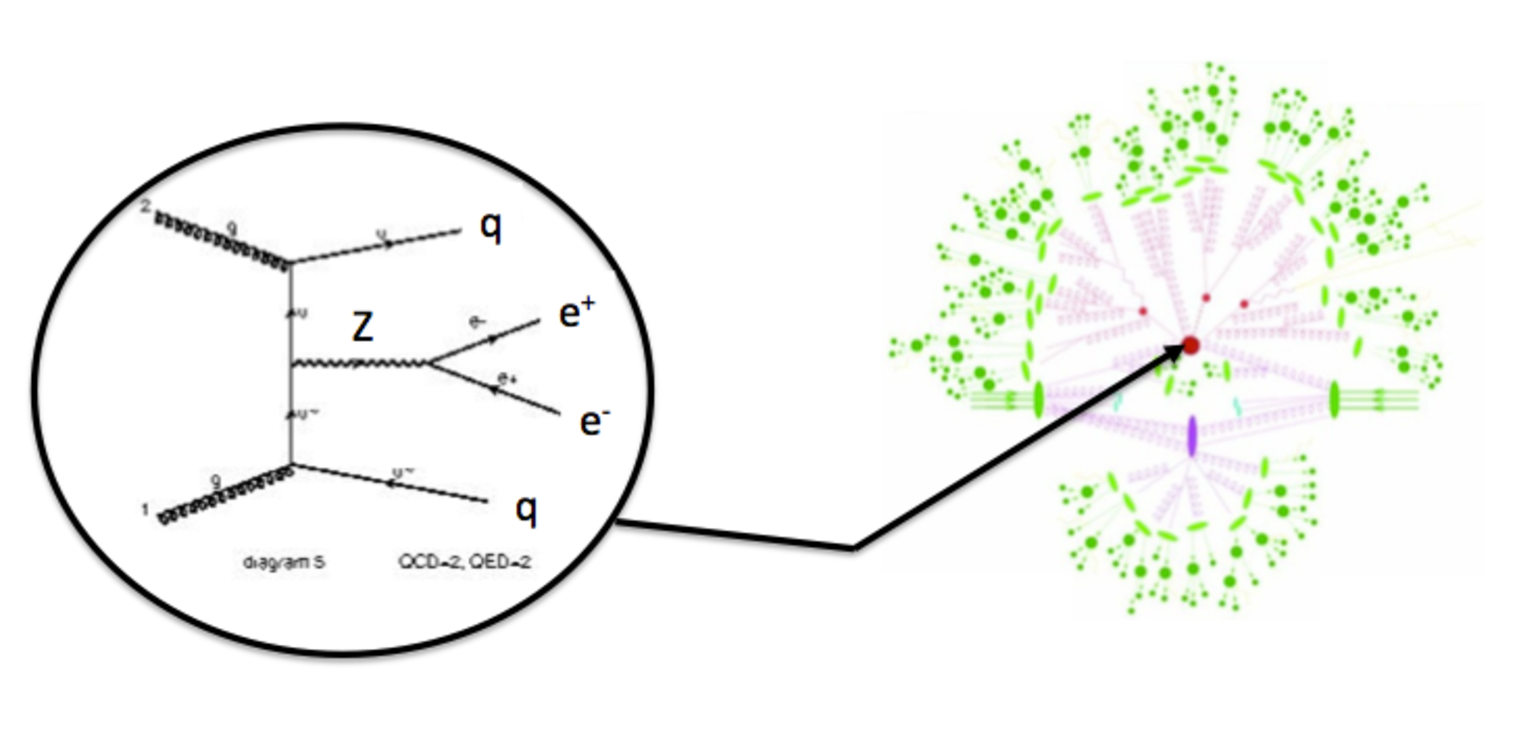
\includegraphics[width=0.9\textwidth]{scatter.pdf}
\caption{Hard scatter by MadGraph on left with subsequent phenomenological showering by Pythia on right.}
  \label{fig:scatter}
\end{figure}
\\
There are many different ways to use it and the procedures presented here are only one path that can be followed and only uses a fraction of its functionality.  It is based on using MadGraph to produce a list of particle 4-vectors coming from the ``hard process" which are then  ``showered" using Pythia ~\cite{pythia} as in Fig~\ref{fig:scatter}.  This showering procedure produces hundreds of ``final state" particles, each of which is represented by a Lorentz 4-vector and would be representative of the particles entering the ATLAS detector.  Because there are so many particles in this final state, these files are formatted in accordance with the Les Houches accord ~\cite{leshouches} into STDHEP files such that they conform to standards of the particle physics community.  There is well-developed software that can read them and put them in terms of a \textit{.root} file that you now know how to analyze from the previous section.  There are two main stages to this conversion.  In the first step, the STDHEP files are transformed to Root readable files using \texttt{ExRootSTDHEPConverter} which creates a Root readable file.  In the second, the file previously produced is sent through an ``nTupler" program to perform the organization of physics objects such as electrons, muons, MET (Missing Transverse Energy), and jets.  In the following, you will learn how to perform each of these steps and how to modify them to suit your needs.

\subsubsection{MadGraph Setup and Usage}
Unless MadGraph is already set up on your machine, you will need to download and install it yourself.  To do so, go to the MadGraph site \href{http://madgraph.hep.uiuc.edu/}{\textit{http://madgraph.hep.uiuc.edu/}}, register yourself as a new user, and go to Downloads to download the latest tarball.  Place it in a working directory and untar it with \\ 
\\
\texttt{prompt> tar -xzvf MadGraph5\_v*\_*\_*}\\ 
\\
Now go into the MadGraph working directory you just created (\textbf{NOTE:} for running MadGraph, you will need a Fortran compiler \texttt{g77}, a c++ compiler \texttt{gcc}, and \texttt{Python v2.6} or later installed on your machine first.)  If you do not have these installed then install them as necessary for your machine.  
Once you have successfully installed the software, start MadGraph and install all four packages, as follows: \\ 
\\
\texttt{prompt-MadGraph> ./bin/mg5}\\
\\
If Python2.6 is not the default version of python for your machine, then modify the first line of the \texttt{./bin/mg5} file from:\\
\texttt{\#! /usr/bin/env python}\\
to:\\
\texttt{\#! /usr/bin/env python26}\\
\\
This will ensure that MadGraph will use the Python2.6 version each time you start it.  If you know that for your machine, there is a different command to set up the the Python2.6 environment, then use this command instead.  Once MadGraph is started, execute:\\
\texttt{
\hspace*{0.0cm}mg5> help install\\
\hspace*{0.0cm}syntax: install pythia-pgs|Delphes|MadAnalysis|ExRootAnalysis\\
\hspace*{0.0cm}-- Download the last version of the program and install it\\
\hspace*{0.4cm}   localy in the current Madgraph version. In order to have\\
\hspace*{0.4cm}   a sucessfull instalation, you will need to have up-to-date\\
\hspace*{0.4cm}   F77 and/or C and Root compiler.\\
\hspace*{0.0cm}mg5> install pythia-pgs\\
} 
\\
and then install Delphes, MadAnalysis, and ExRootAnalysis in the same way.  Wait for each to successfully complete because having each of these is important to be able to output STDHEP files from MadGraph.  Next, in the main MadGraph directory, copy the \texttt{Template} directory to a new directory, call it \texttt{Zjets}.  Go into the \texttt{Zjets/Cards} directory and make sure that all the proper cards are copied as needed.  To get the required STDHEP output, one only needs to copy the pythia card as \\
\\
\texttt{prompt-MadGraph/Zjets/Cards> cp pythia\_card\_default.dat pythia\_card.dat}\\
\\
But, it is also good to have access to other outputs from MadGraph if your analysis needs them in the future, so copy the other cards as \\
\\
\texttt{prompt-MadGraph/Zjets/Cards> cp delphes\_card\_ATLAS.dat delphes\_card.dat }\\
\texttt{prompt-MadGraph/Zjets/Cards> cp delphes\_trigger\_ATLAS.dat delphes\_trigger.dat }\\
\texttt{prompt-MadGraph/Zjets/Cards> cp param\_card\_default.dat param\_card.dat}\\
\texttt{prompt-MadGraph/Zjets/Cards> cp pgs\_card\_ATLAS.dat pgs\_card.dat}\\,
\texttt{prompt-MadGraph/Zjets/Cards> cp proc\_card\_mg5.dat proc\_card.dat}\\
\\
Now that you have all the necessary setup finished, go to your \texttt{Zjets/Cards} directory.  You will be modifying the \texttt{proc\_card\_mg5.dat} file.  This is the card that determines the specific physics process (Feynman diagram) that will be calculated and simulated.  Replace the lines: \\
\\
\texttt{generate p p > e- ve~ @1}\\
\texttt{add process p p > e- ve~ j @2}\\
\texttt{add process p p > t t~ @3 }\\
with:\\
\texttt{generate p p > Z > l+  l-@0}\\
\texttt{add process p p > Z > l+  l- j @1}\\
\texttt{add process p p > Z > l+  l- j j @2}\\ 
\texttt{add process p p > Z > l+  l- j j j@3}\\ 
\\
This indicates that you want to generate three different process, the production of a Z boson (and subsequent decay to $\ell^{+} \ell^{-}$ pair, in association with 0, 1, and 2 jets.  Now modify the \texttt{run\_card.dat} file.  This file controls many different parameters of events you will generate, but to begin with, only change the input beam energies from 7000 (GeV) to 3500 (GeV) to correctly simulate the current LHC beams.
You are now ready to simulate events.  Go into the \texttt{Zjets/} directory and execute: \\
\\
\texttt{prompt-MadGraph/Zjets> ./bin/newprocess\_mg5}\\ 
\\
which will draw all of the corresponding Feynman diagrams for the interaction you specified in the \texttt{proc\_card\_mg5.dat} file.  Now execute :\\ 
\\
\texttt{prompt-MadGraph/Zjets> ./bin/generate\_events}\\ 
\\
entering \texttt{0} to run the event generation in serial and then a descriptive title for the run.  This can be expediated, and later more easily implemented in bash by executing something like:\\ 
\\
\texttt{prompt-MadGraph/Zjets> ./bin/generate\_events 0 Zplus0123jets\_10000events}\\
\\
After MadGraph has finished producing all of the events and the prompt reappears, check the output by executing:\\ 
\\
\texttt{prompt-MadGraph/Zjets> open index.html} \hspace{2cm}Mac  \\ 
\texttt{prompt-MadGraph/Zjets> acroread index.html} \hspace{1cm} Linux\\ 
\\
which will bring you to a web browser and you can view different information about your events.  Explore this page to see what information MadGraph automatically generates.  For instance, by clicking the \textit{Process Information} link, and then a corresponding link to a specific process, one can see all the tree level Feynman diagrams (\textbf{NOTE}: There are no loop diagrams, this is because MadGraph only generates diagrams at tree level, can you guess what this means?)  However, for our purposes, you care about the \textit{Results and Events Database} link.  Go into this link and you will see a number of files that can be downloaded as in Fig~\ref{fig:output}.
\\
\begin{figure}[htp]
\centering
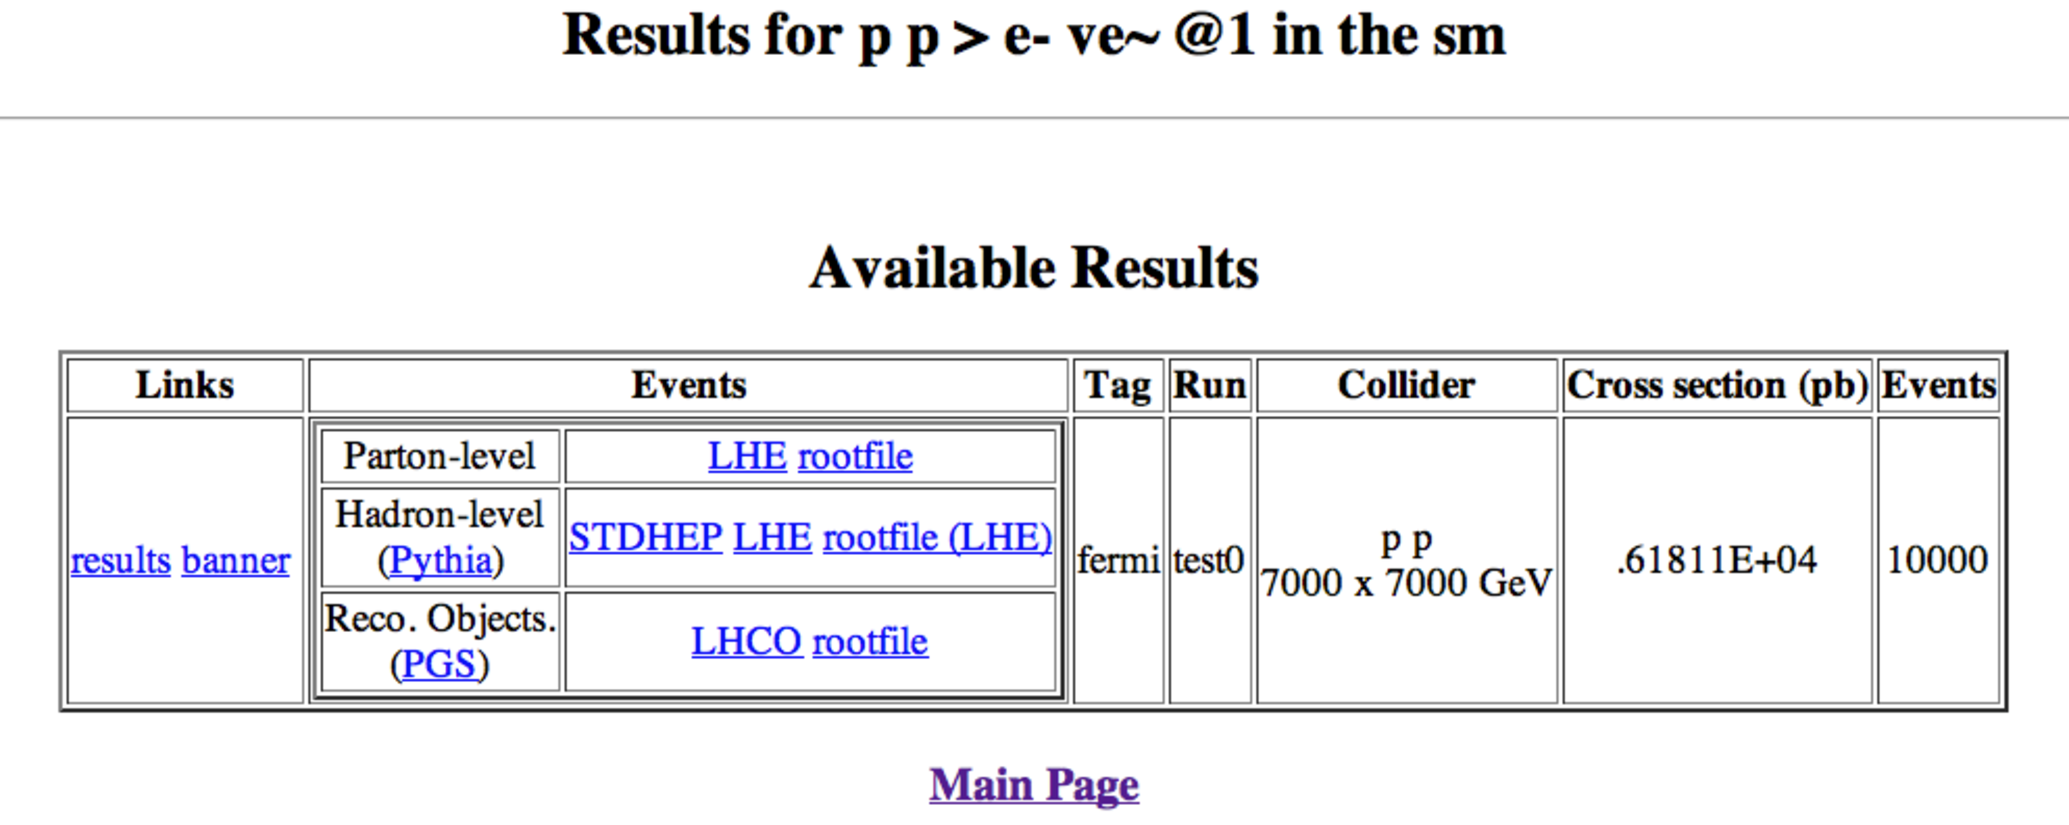
\includegraphics[width=0.9\textwidth]{STDHEPexamples.pdf}
\caption{What the MadGraph page should look like with all the appropriate output if you have installed everything correctly.}
  \label{fig:output}
\end{figure}
\\
Download the STDHEP file corresponding to the process you just generated which is a zipped file ending in the suffix \textit{.hep}. Unzip it and place the and place the \textit{.hep} file into a new directory (call it \texttt{Process}) that will be dedicated to converting and ``nTupling" the files into the format you previously analyzed with Root.  

\subsubsection{ExRootSTDHEPConverter Usage}
If you succesfully installed all the utilities then in the MadGraph directory, there should appear an \texttt{ExRootAnalysis} directory which contains multiple executable files.  Copy the \texttt{ExRootSTDHEPConverter} to the \texttt{Process} directory you created earlier.  Run the STDHEP file through this processor as\\
\\
\texttt{prompt-Process> ./ExRootSTDHEPConverter file\_in.hep file\_out.root}\\ 
\\
to output the Root readable pythia file \texttt{file\_out.root}.  Open this file with a TBrowser and look at its contents to see what information is currently there.  Note though that during the showering process, not all the particles whose kinematics are contained in this file make it to the final state (determined by looking at their \textit{GenParticle.Status}) and enter into the ATLAS detector.  However, all of this information is contained in this file you just produced.  Furthermore, this file contains information on electrons, muon, and photons (all of which we can``measure" 4-vectors for) but also on many other species of particles, identified by their \textit{GenParticle.PID}, that cannot be measured as cleanly, but will be clustered into jets using \texttt{FastJet}.  This process of organizing the Root file you just created, into a file that can be easily analyzed as you previously did, is the topic of the next section.

\subsubsection{FastJet Setup}
The last step in creating an analyzeable ntuple from MadGraph is to transform the showered particle file output from the ExRootSTDHEPConverter into a Root file containing a TTree that, event by event, contains separate banks for the various particle types, their respective 4-vectors, and any other measurement information that may be useful in analysis (e.g. detector quality information - but you probably won't worry about this to begin with).  
To do this you need to start by setting up \texttt{FastJet} which can be found on the web to download at \href{http://fastjet.fr/}{\textit{http://fastjet.fr/}}.  After you have downloaded and unpacked the tarball of the \texttt{FastJet} version you plan to use (I recommend installing version 3 or later to have access to features such as pruning, merging, etc.), download the user manual and follow the quickstart section of the manual, following through until you are able to successfully run the simple example including in the manual.  If you can do this, everything is set up properly.  Note that in the quickstart section of the manual, the main hangup that caused for confusion when trying to compile a program using the FastJet libraries and namespace were that to include the fastjet-install directory, one must be sure to use " ` " (the key in the upper left of the keyboard) instead of an apostrophe " ' ".  \\ 
\subsubsection{nTuple Creation}
After having set up FastJet successfully, go to the site \href{http://hep.uchicago.edu/~meehan/StandaloneAnalysisTutorial/}{\textit{http://hep.uchicago.edu/$\sim$meehan/}} and download the following files:
\begin{itemize}
\item \textbf{MakeFile} : For compiling the nTupler
\item \textbf{NTupleMaker.h} : The main header file for the nTupler containing all the information about the variables in the TTree produced from \texttt{ExRootSTDHEPConverter} and the TTree that will be output from this nTupler, in addition to any other variables, class, or function definition you need for any procedures you write.
\item \textbf{NTupleMaker.cc} : The main nTupler.  This is the piece of the code that will be compiled into an executable and do the conversion of the file from \texttt{ExRootSTDHEPConverter} output into an analyzeable Root TTree.  If you want to add any new routines, or variables to output, this is the file you will use to incorporate these changes.
\item \textbf{ProcessFile.sh} : Bash script that can be run as \\
					   \texttt{prompt-MadGraph/Process> source ProcessFile.sh in.hep out.root}\\
					   to convert a \texttt{.hep} file from MadGraph to a analyzeable output file in one line.
\end{itemize}
The Makefile here includes a directive that includes the \texttt{FastJet} libraries by pointing to the \textit{fastjet-install} directory.  \\
\\
\texttt{FASTJET=/Users/meehan/work/fastjet-install/}\\
\\
To work on your machine, change the path to point the directory in which you created \textit{fastjet-install} earlier.  Now use the Makefile to compile the nTupler (JetClustering) by executing\\ \\ 
 \texttt{prompt-MadGraph/Process> make}\\ \\
which will produce the executeable \texttt{NTupler} which can be run on an input file, \texttt{in.root}, that was previously produced by \textbf{ExRootSTDHEPConverter}, to produce the output nTuple \texttt{out.root}, by executing:\\ \\
\texttt{prompt-MadGraph/Process> ./NTupler in.root out.root}\\
\\
If you have set up all components correctly, this should produce the file \texttt{out.root} which is in the correct format to be analyzed as a Root TTree using the procedure that was previously outlined in the \textbf{Standalone ROOT nTuple Analysis}.\\
\\
If you have done enough Root tutorials and looked at enough examples, you should know the basics of how a Root TTree is structured and how to read/write from it.  If you do not know these at this point, go back and do so, as it will be absolutely necessary if you wish to be able to use this code to investigate new and different kinematics and variables than it currently provides.  Knowing these basics, the best way to understand the code it to read through it line by line and understand what is happenning at each step.  Do this and see if you can identify the following pieces of code and expound on the code by doing the following:
\begin{itemize}
\item Identifying where the program load an event from the input TTree into memory
\item Identifying where the program loops through all the particles in a given event
\item Identifying where the program determines if the particle is a final state particle (based on PID infromation)
\item Identifying where the program creates and fill block corresponding to electrons, muons, and photons.  These two things may happen in two different locations.
\item Where MET (Missing Transverse Energy) is calculated.  Does this calculation make sense?
\item What does the nTupler do with the leftover particles that are identified as being in the final state, but not idenitified as electrons, photons, or muons?  FastJet is invoked here to create variable blocks corresponding to different \textit{jet collections}.  Currently there are blocks corresponding AntiKt7 and AntiKt10 jets, see if you can create a block with the same structure of AntiKt4 jets and one for Cambridge-Aachen jets.  If these terms seem foreign to you, then go back to FastJet and work through some of the tutorials, they will help explain the nuts and bolts of how to get FastJet to do different things.  And then ask someone what these different jets are.
\end{itemize}

\subsection{Standalone ROOT nTuple Analysis}
\footnote{The steps presented here are adapted from the tutorial \href{https://wiki.physik.uni-muenchen.de/etp/index.php/ROOT_grid_analysis}{\textit{https://wiki.physik.uni-muenchen.de/etp/index.php/ROOT\_grid\_analysis}} }
To perform standalone analysis, you will be using the c++ coding language.  One of the main websites with directions on how to use different features of this language is \href{http://www.cplusplus.com/}{\textit{http://www.cplusplus.com/}}.  The official root website can be found at \href{http://root.cern.ch/drupal/}{\textit{http://root.cern.ch/drupal/}}.  This contains documentation that will be useful as you progress and want to use more complicatted tools from Root.  The conventional way to do analysis with root is to use something called the TSelector class, which can be run within Root to perform a set of event selections.  However, in this framework, you will create a class (\texttt{Physics}) to analyze ntuples that can be used as a standalone, compileable program that draws upon functionality from \texttt{Root} and \texttt{FastJet}.

\subsubsection{Initial Setup}
Before analysis, follow these steps to get c++ and Root set up on your machine.  This is easier to do for Linux or Mac machines.  If you have a Windows machine, we reccomend that you partition your hard drive and install Linux on part of your hard drive. This way, you can use the Linux part of you machine to boot into the environment that can be used for analysis.  If you are working on a UChicago HEP computer, these utilities are likely setup for you already.  
\begin{itemize}
\item If you do not know how to program in c++, start by performing a few basic tutorials to learn how to write compileable programs and use Makefiles.  Such tutorials can be found on \href{http://www.cplusplus.com/doc/tutorial/}{\textit{http://www.cplusplus.com/doc/tutorial/}}
\item If you do not already have Root set up on your machine and/or do not know how to use it then start by downloading and installing the latest version of Root on your machine.  This is described on \textit{http://root.cern.ch/drupal/content/downloading-root}.  
\item After installing Root, go to the page \href{http://root.cern.ch/drupal/content/downloading-root}{\textit{http://root.cern.ch/root/html/tutorials/} }.  There are many directories here that have ``tutorials" based around different functionalities of Root.  These are not tutorials as you (should have) worked through previous to the MadGraph section of this, but they are more pieces of code that can be executed independently to do a specific task in Root.  These are useful as tools to take code peices from in the future.  For now, just look at a few of the examples in the ``hist" directory concerning Histograms and how to draw them.  After that, it may be useful to also look at the ``tree" directory and a few of the basic tutorials to see how to write an NTupler from scratch by inputting your own data.  (A diligent student would work through as many as possible, but at some point your eyes may start to bleed, and that is no good)
\item After you are comfortable with Root, you will use an automatic Root utility to create a standalone ``class" (you should know what this is in c++ speak) that can be compiled and run to analyze an ntuple.  This is described in the next section.
\end{itemize}

\subsubsection{Generate Class} 
Start by obtaining a Root ntuple that has the structure of a TTree (a Root class).  One such example of an nTuple can be found at \\
\\ 
\href{http://hep.uchicago.edu/$\sim$meehan/StandaloneAnalysisTutorial/}{\textit{http://hep.uchicago.edu/$\sim$meehan/}
\\
\href{http://hep.uchicago.edu/$\sim$meehan/StandaloneAnalysisTutorial/}}{\textit{StandaloneAnalysisTutorial/}}
\\
with the suffix of \textit{.root}.  This is the same format of nTuple as you will be producing in the next section of this tutorial, using \texttt{MadGraph}.  Download this and put it in a directory of your own called it \textit{MyAna}. Change directories into the MyAna director, open root and use it to create the Physics.h and Physics.C class files.\\ \\
\texttt{root [1] TFile *f = new TFile("ZZWZ\_llqq\_10000events\_ntuple\_01.root")} \\
\texttt{root [2] TTree *t = (TTree*)f->Get("Physics")} \\
\texttt{root [3] t-$>$MakeClass("Physics")} \\
\texttt{Info in $<$TTreePlayer::MakeClass$>$: Files: Physics.h and Physics.C generated from TTree: Physics}\\
\texttt{(Int\_t)0}\\

\subsubsection{Modify Physics.h} 
Now that you have created the basic analysis class using root, you must modify the necessary sections to make it a program that can be compiled as a standalone program and used to analyze the ntuple (\textbf{or any ntuple with the same structure}) without Root.  The first piece you will modify is the \textit{header} file \textbf{Physics.h}.  \\
\\
At the top of the header file, folling the \texttt{\#define} line, include the following lines:\\
\texttt{
\#include $<$iostream$>$\\
\#include "TFileCollection.h"\\
using namespace std;\\
}
\\
Replace:\\
\texttt{TTree          *fChain;   //!pointer to the analyzed TTree or TChain}\\
By:\\
\texttt{TChain         *fChain;  //!pointer to the analyzed TTree or TChain}\\\\
Replace:\\
\texttt{Physics(TTree *tree=0);}\\
By:\\
\texttt{TChain* chain;}\\
\texttt{Physics(const char* fileName);}\\\\
Note that this is where one can include the declarations of extra functions you need in your .C file ( e.g. \texttt{int elec\_selection(int ielec); } for selecting a subset of good electrons).  It is alright if you don't have any of these yet, however, if you don't know how to declare functions in c++, you may want to go back to your c++ tutorials and review how to do this at this point.\\
\\
Replace the \textit{constructor} (another c++ word you should know associated to classes):\\
\texttt{
\hspace*{0.0cm}Physics::Physics(TTree *tree)\{ \\
\hspace*{0.2cm}// if parameter tree is not specified (or zero), connect the file\\
\hspace*{0.2cm}// used to generate this class and read the Tree.\\
\hspace*{0.2cm}if (tree == 0)\{\\
\hspace*{0.4cm}TFile *f = (TFile*)gROOT->GetListOfFiles()\\
\hspace*{2.6cm}->FindObject("ZZWZ\_llqq\_10000events\_ntuple\_01.root");\\
\hspace*{0.4cm}if(!f)\{\\
\hspace*{0.6cm}f = new TFile("ZZWZ\_llqq\_10000events\_ntuple\_01.root");\\
\hspace*{0.4cm}\}\\
\hspace*{0.4cm}tree = (TTree*)gDirectory->Get("physics");\\
\hspace*{0.2cm}\}\\
\hspace*{0.2cm} Init(tree);\\
\hspace*{0.0cm}\}}
\\
By the constructor:\\
\texttt{
\hspace*{0.0cm}Physics::Physics(const char* inputFile)\{ \\
\hspace*{0.2cm}TChain * chain = new TChain("Physics","");\\
\hspace*{0.2cm}TFileCollection* fc = new TFileCollection("mylist", "mylist",inputFile);\\
\hspace*{0.2cm}chain->AddFileInfoList((TCollection*)fc->GetList());\\
\hspace*{0.2cm}std::cout << "Total  number of entries in chain (all files) " \\
\hspace*{2.4cm}<<  chain->GetEntries() << std::endl;\\
\hspace*{0.2cm}Init(chain);\\
\hspace*{0.0cm}\}\\
}
\\
Replace:\\
\texttt{void Physics::Init(TTree *tree)}\\
By:\\
\texttt{void Physics::Init(TChain *tree)}\\\\
Replace:\\
\texttt{virtual void \hspace{0.5cm}     Init(TTree *tree);}\\
By:\\
\texttt{virtual void \hspace{0.5cm}     Init(TChain *tree);}\\
\\
\newpage
\subsubsection{Modify Physics.C} 
Start by including the basic headers one needs to do analysis with the Root tools include the headers you need for your analysis:\\
\texttt{ 
\#include $<$TROOT.h$>$\\
\#include $<$TChain.h$>$\\
\#include $<$TFile.h$>$\\
\#include $<$TH1.h$>$\\
\#include "TApplication.h"            //mandatory\\
\#include $<$stdio.h$>$\\
\#include $<$stdlib.h$>$\\
\#include $<$iostream$>$\\
\#include $<$fstream$>$\\
\#include $<$math.h$>$\\
\#include $<$vector$>$\\
\#include $<$list$>$\\
\#include $<$string$>$\\
}
\\
Include the following function just below the \texttt{\#include} statements.  Note that the ``input.txt" file contains a newline separated list of the ntuple files over which you want to run the analysis code.  You will create this file with a sample nTuple path later.\\
\texttt{
\hspace*{0.0cm}int main(int argc, char **argv)\\
\hspace*{0.0cm}\{  \\
\hspace*{0.4cm}Physics a("input.txt"); //instance "a" of Physics with input.txt files\\
\hspace*{0.4cm}a.Loop(); \hspace{3cm}//execute code in Loop() function of "a"\\
\hspace*{0.0cm}\}\\
}
\\
The main part of the analysis will be done in the \texttt{Physics::Loop()} function.  From what you know from doing the root tutorials, you will be able to implement things as below.  Start by removing all the comment lines and replace the remaining code with the modified code below.  \\
\texttt{
\hspace*{0.0cm}TH1F* h1 = new TH1F("h1","electron pt",1000,0,1000);\\
\hspace*{0.0cm}if (fChain == 0) return;\\
\hspace*{0.0cm}Long64\_t nentries = fChain->GetEntriesFast();\\
\hspace*{0.0cm}Long64\_t nbytes = 0, nb = 0;\\
\hspace*{0.0cm}for (Long64\_t jentry=0; jentry<nentries; jentry++)\{\\
\hspace*{0.4cm}   Long64\_t ientry = LoadTree(jentry);\\
\hspace*{0.4cm}   if (ientry < 0) break;\\
\hspace*{0.4cm}   nb = fChain->GetEntry(jentry);   nbytes += nb;\\
\hspace*{0.4cm}   if(el\_n>0)\{\\
\hspace*{0.8cm}	     h1->Fill(el\_pt->at(0));\\
\hspace*{0.4cm}   \}\\
\hspace*{0.0cm}\}\\
\hspace*{0.0cm}TFile outputfile("Physics\_output.root","RECREATE");\\
\hspace*{0.0cm}h1->Write();\\
\hspace*{0.0cm}outputfile.Close();\\
}
\\
This is only a brief example and fills the histogram with the $p_{T}$ of only the first electron in each event.  Over time, your analysis will grow by adding things like this.  After adding a few basic things to (1) create, (2) fill, and (3) writeout histograms for various variables, move on to the next section.\\

\subsubsection{Make Compiling Tools} 
In the directory you have been working to create your analysis code make a new textfile called ``Makefile" and copy the following lines to it.  This is your \textit{Makefile} (something you have hopefully learned about from your exploration of c++.  This is used to compile your analysis into an executable file and link to this any external libraries necessary to do complicated things like scaling measured electron energies to account for detector defects or calculating reweighting factors that account for something called \textit{pileup} (if you don't know what this is, ask someone).  You will most like not have to deal with such things right away, but having the ability to do so will help you convert your analysis code into something that can more easily be used to do ATLAS analysis.\\
\texttt{\\
\hspace*{0.0cm}ROOTCFLAGS := \$(shell root-config --cflags)\\
\hspace*{0.0cm}ROOTLIBS := \$(shell root-config --libs) -lMinuit -lEG\\
\hspace*{0.0cm}\\
\hspace*{0.0cm}CXX := g++\\
\hspace*{0.0cm}CXXFLAGS := -O -Wall -fPIC \$(ROOTCFLAGS)\\
\hspace*{0.0cm}OBJS := Physics.o\\
\hspace*{0.0cm}\\
\hspace*{0.0cm}Physics : \$(OBJS)\\
\hspace*{0.3cm}    \$(CXX) -o \$@ \$(OBJS) \$(CXXFLAGS) \$(ROOTLIBS)\\
\hspace*{0.0cm}\\
\hspace*{0.0cm}.cc.o :\\
\hspace*{0.3cm}    \$(CXX) -c \$(CXXFLAGS) \$<\\
\hspace*{0.0cm}\\
\hspace*{0.0cm}clean :\\
\hspace*{0.3cm}    rm -f *.o\\
}\\
Note that in this code, the lines indented must be indented using a \textit{tab} and not a string of spaces or the Makefile will not run properly.  \\
\\
Now make a new textfile called ``input.txt" and copy the name of the test dataset files to it as below. Make a line break after each dataset file.  Note that these datasets can reside in any location and you must just provide the entire path to the dataset if they are not in the same directory as your analysis code.  If the file resides in the same directory as your analysis code, they you use \\
\texttt{ZZWZ\_llqq\_10000events\_ntuple\_01.root} \\
but if it does not, then you would use \\ \texttt{datasets/mysets/montecarlo/signal/ZZWZ\_llqq\_10000events\_ntuple\_01.root}\\
if they reside in the directory \textit{datasets/mysets/montecarlo/signal}.  And as before, if you have multiple files you want to string together and run in the same analysis, then you can include their paths as new lines in this file.  However, do not mix physics processes!  One should only need to link together multiple files when they are limited by the number of events that can be stored in a single file for a single process.

\subsubsection{Compile and Run for First Time} 
After making the previous files, you are ready to run your analysis code.  To compile the code type:\\
\\
\texttt{prompt$>$ make}\\
\\
Be patient, this may take a while, and will take longer if you have an involved code, or you are including multiple external libraries.  Chances are you will have bugs in your code, and you will need to fix these.  However, once the code is compileable, this will produce an output executable \textit{Physics}.  If everything has been done correctly to this point and you have this executable, then the executable can be run by typing: \\ 
\\
\texttt{prompt$>$ ./Physics}\\ 
\\
This will run your analysis code, creating and filling any histograms you have specified it to, and printing out any messages you have specified it to print.  It should produce the output file \textit{Physics\_output.root} that you told it to above.  As you should know from the Root tutorials, this file and its contents can be viewed by running root:\\ 
\\
\texttt{root[0] new TBrowser}\\ 
\\
If you have done everything correctly, then this file should contain some histograms of various things you have specified.  You're job now is to figure out if these histograms are "correct" (Are they filled? Do they have the right shape?  Do they have too many bins? Too few?) and then elaborate on your code to produce histograms of different variables, with different kinematic selections to investigate the different aspects of the physics in which you are interested.  Some things you may want to consider adding to your code at this point, to allow for more flexibility, if you have not done so already, are:
\begin{itemize}
\item The ability to pass the executable arguments (look up how to do this in the c++ reference).  This will allow you to pass it a \textit{char*} argument that specifies which set of input files to run over so that it can be made to analyze signal or background.  You can also specify the name of the output \textit{.root} file this same way so the output is different for signal or background.
\item A loop that runs over all events in the data file.
\item A section (it could be an external function or class if you know how to do this) that selects electrons, muon, and/or jets that pass certain kinematic (or quality) requirements like $p_{T}(electron)>30.0$ GeV.  This would have to be run for each electron in each event.
\item A conditional statement that only selects events that have \textit{exactly two good (as defined above), oppositely charged} leptons and combines their four vectors into a single four vector representative of a dilepton (Z boson in some cases) system.  Try exploring the \textit{TLorentzVector} class in Root to do this.
\end{itemize}



\section{Encouraging Words}
When doing data analysis there seem two be to main hurdles that you encounter:
\begin{enumerate}
\item "Why doesn't anything work?"
\item "Why is this so damn hard?"
\end{enumerate}
Hopefully this short guide has helped to adress the first and allow you to concentrate more on the second over the coming days, weeks, and months.  Good luck!

\bibliographystyle{plain}	% (uses file "plain.bst")
\bibliography{myrefs}		% expects file "myrefs.bib"

\end{document}

\end{document}


